\chapter{Analisi}

\section{Descrizione e requisiti}

Il software mira alla alla costruzione di una versione virtuale del famoso gioco da tavolo “Monopoly”. 
Quest’ultimo è un gioco di società nel quale più giocatori si muovono a turni su di un tabellone 
composto da caselle differenti con lo scopo di creare un monopolio. 
Durante la partita i giocatori si scambiano denaro a vicenda sotto 
forma di pagamenti e possono acquistare e migliorare proprietà. 
L’obiettivo è mandare gli altri giocatori in bancarotta, vince l’ultimo giocatore rimasto. 




\subsection*{Requisiti funzionali}
\begin{itemize}
    \item Il gioco potrà essere giocato su uno stesso dispositivo da un minimo di 2 giocatori ed un massimo di 6.
	\item Il giocatore potrà tirare i dadi per far muovere la propria pedina sul tabellone.
	\item Durante il proprio turno ciascun giocatore avrà la possibilità di acquistare la proprietà sulla quale 
    si trova se di proprietà della banca, altrimenti pagare l’affitto al proprietario. 
    Ci saranno anche delle caselle speciali con effetti specifici.
    \item Nel corso della partita un giocatore, quando capita sulle sue proprietà, le potrà migliorare spendendo
    del denaro per posizionare delle case che elevano il costo dell’affitto.
    \item Durante il proprio turno, se lo desidera, il giocatore potrà vendere alla banca 
    le proprietà o eventuali case presenti su esse.
\end{itemize}


\subsection*{Requisiti non funzionali}
\begin{itemize}
    \item modularità azioni
    \item salvare su file lo storico dei risultati delle partite precedenti
    \item interfaccia grafica responsive
    \item caricare metadata (dati delle caselle) da file locale
    \item rendere l’applicazione portabile su più SO
\end{itemize}

\section{Modello del dominio}
Il sistema (TurnationManager) deve gestire l’avvicendarsi dei vari turni dei giocatori. 
A ogni giocatore (Player) viene concesso periodicamente il proprio turno d’azione sulla base di una rotazione ciclica. 
Durante il turno il giocatore tira i dadi e si muove sul tabellone (Board) finendo sempre su una casella (Card).
Questa casella può essere una proprietà (Property) oppure una casella speciale (Special), 
e sulla base di ciò cambia radicalmente l’interazione dell’utente. 
Se capita su una proprietà che non è ancora posseduta da alcun giocatore allora 
il giocatore può decidere di acquistarla. 
Se invece la proprietà è già stata comprata si possono verificare due casistiche: il proprietario è un 
altro giocatore, il proprietario è il giocatore che sta svolgendo il proprio turno. 
Nel primo caso il giocatore è obbligato a pagare l’affitto al proprietario, 
nel secondo caso può decidere se migliorare la sua proprietà aggiungendo case.
Se capita su una casella speciale invece si attiverà un effetto caratteristico 
per ognuna di loro che avrà ripercussioni sullo svolgimento del gioco 
(guadagno/perdita denaro, saltare un determinato numero di turni, affrontare sfide)
Una volta che il giocatore avrà svolto tutte le azioni obbligatorie potrà decidere di terminare il proprio turno. 
Fatto questo se il suo saldo è in negativo perde la partita e tutte le sue proprietà tornano disponibili per l’acquisto. 




\begin{figure}[H]
    \centering
    \makebox[1.0\textwidth]{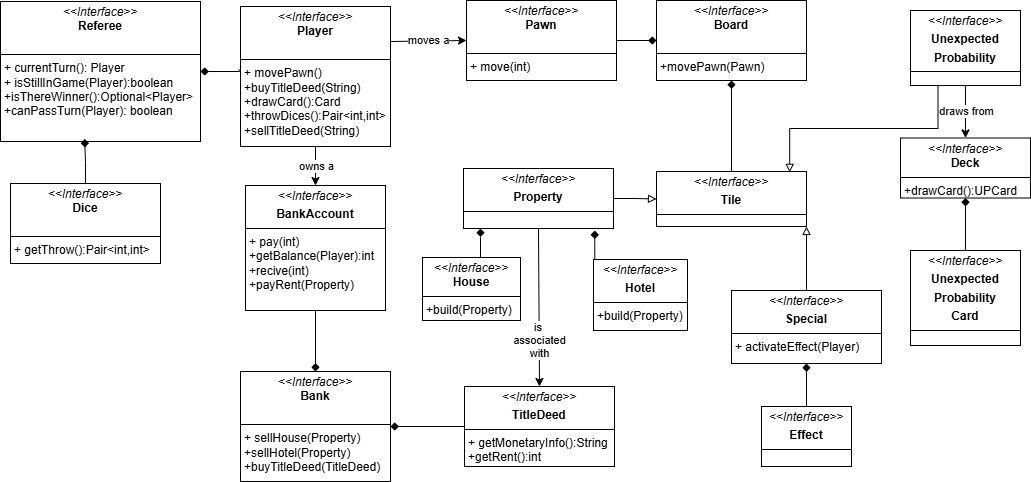
\includegraphics[width=1.5\textwidth]{img/entity_diagram.png}}	
    \caption{Schema UML dell'analisi del problema, con rappresentate le entità principali ed i rapporti fra loro}
	\label{img:entity_diagram}
\end{figure}
